\documentclass[letter]{article}
\usepackage[utf8]{inputenc}
\usepackage[margin=1in]{geometry}
\usepackage{tikz}
\usepackage{ulem}
\usepackage{graphics}
\usepackage{sidecap}
\usepackage{wrapfig}
\usepackage[toc,page]{appendix}
\usepackage{caption}
\usepackage{amssymb}
\usepackage{amsmath}
\usepackage{algorithmicx}
\usepackage{algpseudocode}

\usepackage{url,graphicx,tabularx,array,geometry,amsmath,tikz}
\usepackage{algorithm}% http://ctan.org/pkg/algorithms
\usepackage{algpseudocode}% http://ctan.org/pkg/algorithmicx
\usepackage{listings}
\usetikzlibrary{arrows}
\newenvironment{myindentpar}[1]% %indent whole paragraph when needed
 {\begin{list}{}%
         {\setlength{\leftmargin}{#1}}%
         \item[]%
 }
 {\end{list}}

\usepackage{hyperref}
\usepackage{parskip}

\lstset{
  basicstyle=\small,
  stringstyle=\ttfamily,
  numbers=left,
  numberstyle=\tiny,
  stepnumber=1, 
  numbersep=5pt,
  language=R }

\hypersetup{
    colorlinks,%
    citecolor=black,%
    filecolor=black,%
    linkcolor=black,%
    urlcolor=black
}

\def\dashuline{\bgroup 
  \ifdim\ULdepth=\maxdimen  % Set depth based on font, if not set already
	  \settodepth\ULdepth{(j}\advance\ULdepth.4pt\fi
  \markoverwith{\kern.15em
	\vtop{\kern\ULdepth \hrule width .3em}%
	\kern.15em}\ULon}
\setlength\parindent{2em}

\newcounter{foot}
\setcounter{foot}{1}

\author{Olga Prilepova, Christopher Patton, Alexander Rumbaugh, \\ John Chen, Thomas Provan}

\date{\today}
\title{ECS256 - Homework II}
	
\begin{document}
\maketitle


%%%%%%%%%%%%%%%%%%%%%%%%%%%%%%%%%%%%%%%%%%%%%%%%%%%%%%%%
\subsection*{Problem 1} 

As suggested by the hint, in order to find the bias at $t=0.5$, we're going to be examining the value of $\beta$ as n goes to $\infty$. The idea behind this is that the proposed model will converge to some $\beta$ as the number of samples increases, to the point that it fits as closely as possible to the actual function. Of course, it isn't possible for the model to fit precisely, because the actual relationship isn't linear like the model is, so there will be some bias in the resulting model. 

The first thing to consider is model construction. The simplest way to construct the model would be to use a least-squares method, so in the construction we would  minimize the following with respect to $g(X)$, which is the set of all possible functions for our model.

\begin{equation}
	E[(EY - g(X))^2]
\end{equation}

For this problem, $g(X)=\beta X$ for all possible $\beta$, and the actual distribution of $EY$ is $X^{0.75}$, so we can rewrite this to minimizing the following with respect to $\beta$

\begin{equation}
	E[(X^{0.75} - \beta X)^2]
\end{equation}

To actually find this value, we will first make a new variable $Q=(X^{0.75} - \beta X)^2$, and then use the continuous case of iterated expectations along X (eq 5.33) to find $EQ$

\begin{equation}
	EQ = \int _{-\infty} ^\infty f_X(t) \; E(Q | X = t)\; dt
\end{equation}

\begin{equation}
	E(Q | X = t) = E[(t^{0.75} - \beta t)^2] = (t^{0.75} - \beta t)^2
\end{equation}

X is $U(0,1)$, so $f_X(t)$ is 1 between the values of 0 and 1, and is zero elsewhere. With this and the value of $E(Q | X = t)$, we can rewrite $EQ$ as the following.

\begin{equation}
	EQ = \int _0 ^1 (t^{0.75} - \beta t)^2 \; dt
\end{equation}

From here it's a simple matter to minimize with respect to $\beta$. First, finish computing the integral to get the final function of $\beta$ to minimize.

\begin{equation}
	EQ = \frac{1}{3}(\beta^2 - \frac{24}{11}\beta + \frac{6}{5})
\end{equation}

And then take the derivative of the function with respect to $\beta$.

\begin{equation}
	\frac{d\,EQ}{d\beta} = \frac{2}{3}\beta - \frac{8}{11}
\end{equation}

And finally set that equal to zero and solve for $\beta$, which yields $\beta=\frac{12}{11}$ as the value that minimizes our function.

Now we can move on and compute the bias. The bias is simply $\hat{m}_{Y;X}(t) - m_{Y;X}(t)$, which for the selected $\beta$ and $t=0.5$ is

\begin{equation}
	Bias(0.5) = \beta 0.5 - 0.5^{0.75} \approx {\fbox {\parbox{0.5in}{-0.0491}}}
\end{equation}

%%%%%%%%%%%%%%%%%%%%%%%%%%%%%%%%%%%%%%%%%%%%%%%%%%%%

\subsection*{Problem 2.a\footnote{See \texttt{Parsimony.R} in the project folder.}}






%\lstinputlisting{figures/prsm_fig.R}


\subsection*{Problem 2.c}
Our next data set explores house value throughout California derived from 1990 census data. The state is divided up into 20640 geographic blocks with average population 1425.

We are interested in how the following variables affect median house value: median income, housing median age, total rooms, total bedrooms, population, households, latitude, and longitude.

Here is R's summary output of the data:
\begin{verbatim}
Median.House.Value Median.Income       Median.Age   
 Min.   : 14999     Min.   : 0.4999   Min.   : 1.00  
 1st Qu.:119600     1st Qu.: 2.5634   1st Qu.:18.00  
 Median :179700     Median : 3.5348   Median :29.00  
 Mean   :206856     Mean   : 3.8707   Mean   :28.64  
 3rd Qu.:264725     3rd Qu.: 4.7432   3rd Qu.:37.00  
 Max.   :500001     Max.   :15.0001   Max.   :52.00
Total.Rooms    Total.Bedrooms     Population   
 Min.   :    2   Min.   :   1.0   Min.   :    3  
 1st Qu.: 1448   1st Qu.: 295.0   1st Qu.:  787  
 Median : 2127   Median : 435.0   Median : 1166  
 Mean   : 2636   Mean   : 537.9   Mean   : 1425  
 3rd Qu.: 3148   3rd Qu.: 647.0   3rd Qu.: 1725  
 Max.   :39320   Max.   :6445.0   Max.   :35682
 Households        Latitude       Longitude     
 Min.   :   1.0   Min.   :32.54   Min.   :-124.3  
 1st Qu.: 280.0   1st Qu.:33.93   1st Qu.:-121.8  
 Median : 409.0   Median :34.26   Median :-118.5  
 Mean   : 499.5   Mean   :35.63   Mean   :-119.6  
 3rd Qu.: 605.0   3rd Qu.:37.71   3rd Qu.:-118.0  
 Max.   :6082.0   Max.   :41.95   Max.   :-114.3  
 \end{verbatim}

 
 Next we use our Parsimony package on the data at various k levels. Here are the calls and output:
\begin{verbatim}
 > prsm(df[,1],df[,2:9],k=0.01, predacc=ar2, crit='max', printdel=T)
full outcome =  0.6369649 
deleted         Total.Rooms 
new outcome  =  0.6350863 
deleted         Total.Bedrooms 
new outcome  =  0.6321316 
[1] "Median.Income" "Median.Age"    "Population"    "Households"    "Latitude"      "Longitude"
\end{verbatim}
\begin{verbatim}
> prsm(df[,1],df[,2:9],k=0.05, predacc=ar2, crit='max', printdel=T)
full outcome =  0.6369649 
deleted         Median.Age 
new outcome  =  0.6243571 
deleted         Total.Rooms 
new outcome  =  0.6218261 
deleted         Total.Bedrooms 
new outcome  =  0.6198323 
[1] "Median.Income" "Population"    "Households"    "Latitude"      "Longitude"
 \end{verbatim}
By loosening our k value, the model selector decides to remove Median Age in the latter run. It is interesting to note that longitude and latitude remain in the model, which we will address later.

Next we want to compare our Parsimony package to the significance testing approach. 

Here is the summary of the coefficients of our lm() call in R:
\begin{verbatim}
Coefficients:
                 Estimate Std. Error t value Pr(>|t|)    
(Intercept)    -3.594e+06  6.254e+04 -57.468  < 2e-16 ***
Median.Income   4.025e+04  3.351e+02 120.123  < 2e-16 ***
Median.Age      1.156e+03  4.317e+01  26.787  < 2e-16 ***
Total.Rooms    -8.182e+00  7.881e-01 -10.381  < 2e-16 ***
Total.Bedrooms  1.134e+02  6.902e+00  16.432  < 2e-16 ***
Population     -3.854e+01  1.079e+00 -35.716  < 2e-16 ***
Households      4.831e+01  7.515e+00   6.429 1.32e-10 ***
Latitude       -4.258e+04  6.733e+02 -63.240  < 2e-16 ***
Longitude      -4.282e+04  7.130e+02 -60.061  < 2e-16 ***
--- 
\end{verbatim}
The significance testing approach deletes no predictors. This data set has a large size (20640) so it makes sense that the predictors are all deemed significant.

Here is a summary of the comparison of methods:

\begin{tabular}{ | c | p{3cm} | p{3cm} | c  |}
\hline
Method&Parsimony (k=0.01) & Parsimony (k=0.05) & Significance Testing \\
\hline
Columns\newline Deleted& Total Rooms \newline Total Bedrooms & Total Rooms \newline Total Bedrooms \newline Median Age & None \\
\hline
Adjusted RSquared & 0.6321316 & 0.6218261 & 0.6369649 \\
\hline
\end{tabular}

Before discussing conclusions about the data, we address latitude and longitude. Looking at the full summary above, latitude and longitude both have negative coefficient values. This says if we travel east or north, on average house value decreases. However a real estate expert would think you are crazy hearing that statement.

The problem arises with using coordinate data in a linear regression model. Without any interaction terms we are assuming the statement above. We would risk overfitting if we attempted to make a complex formula involving coordinates. 

A block's location is clearly important. We can see what blocks are close to one another, and proximity to oceans or mountains. Using location data effectively can lead to powerful models, however our model is not set up to do this. But we can plot our data atop a map which we will show shortly.

We remove latitude and longitude and use the predictors kept by our Parsimony package. Here is the summary of the regression:
\begin{verbatim}
Coefficients:
                Estimate Std. Error t value Pr(>|t|)    
(Intercept)   -32165.268   2167.358  -14.84   <2e-16 ***
Median.Income  43094.918    284.263  151.60   <2e-16 ***
Median.Age      2000.544     45.080   44.38   <2e-16 ***
Population       -43.045      1.127  -38.20   <2e-16 ***
Households       152.700      3.344   45.66   <2e-16 ***
\end{verbatim}
First we see that income positively affects house value which is unsurprising. If people have more income, they can afford more expensive houses.

Next looking at age, we see it also positively affects house value. One would expect older people to have more money and this reflected in the high co-variance between these predictors.

Moving onto population, we see it negatively affects house value. With this data set each block has approximately similar geographic size, so blocks with higher population can be assumed to be denser. From our model we can conclude less dense areas have higher housing value. 

Finally we look at number of households which positively affects house value. This is a bit surprising since population had a negative coefficient. One possible explanation is that our model is detecting large suburban areas which are all houses. Areas with more apartment complexes would fewer number of households and also lower housing value.

Parsimony simplified our model down to four predictors. While we lost the data about rooms, we still have a model we can clearly understand.  

Now we make use of our coordinate data using R's ggmap library. First we looked at a map of California as a whole, then zoomed into the Bay Area and the Greater Los Angeles area.

\newpage
\begin{figure}[H]
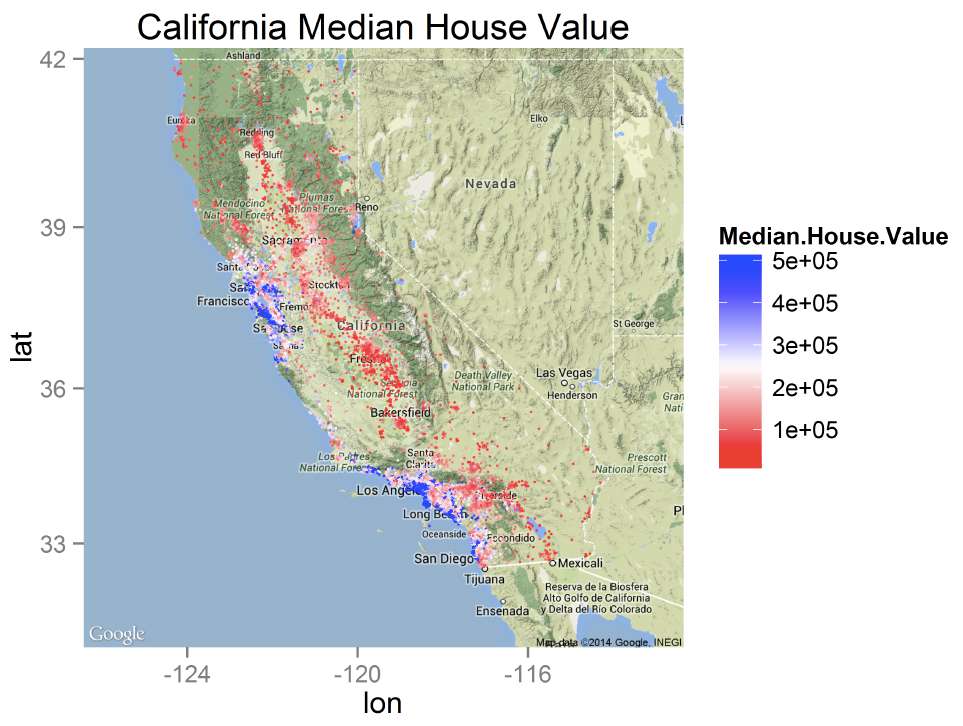
\includegraphics[scale=.54]{figures/california.png}
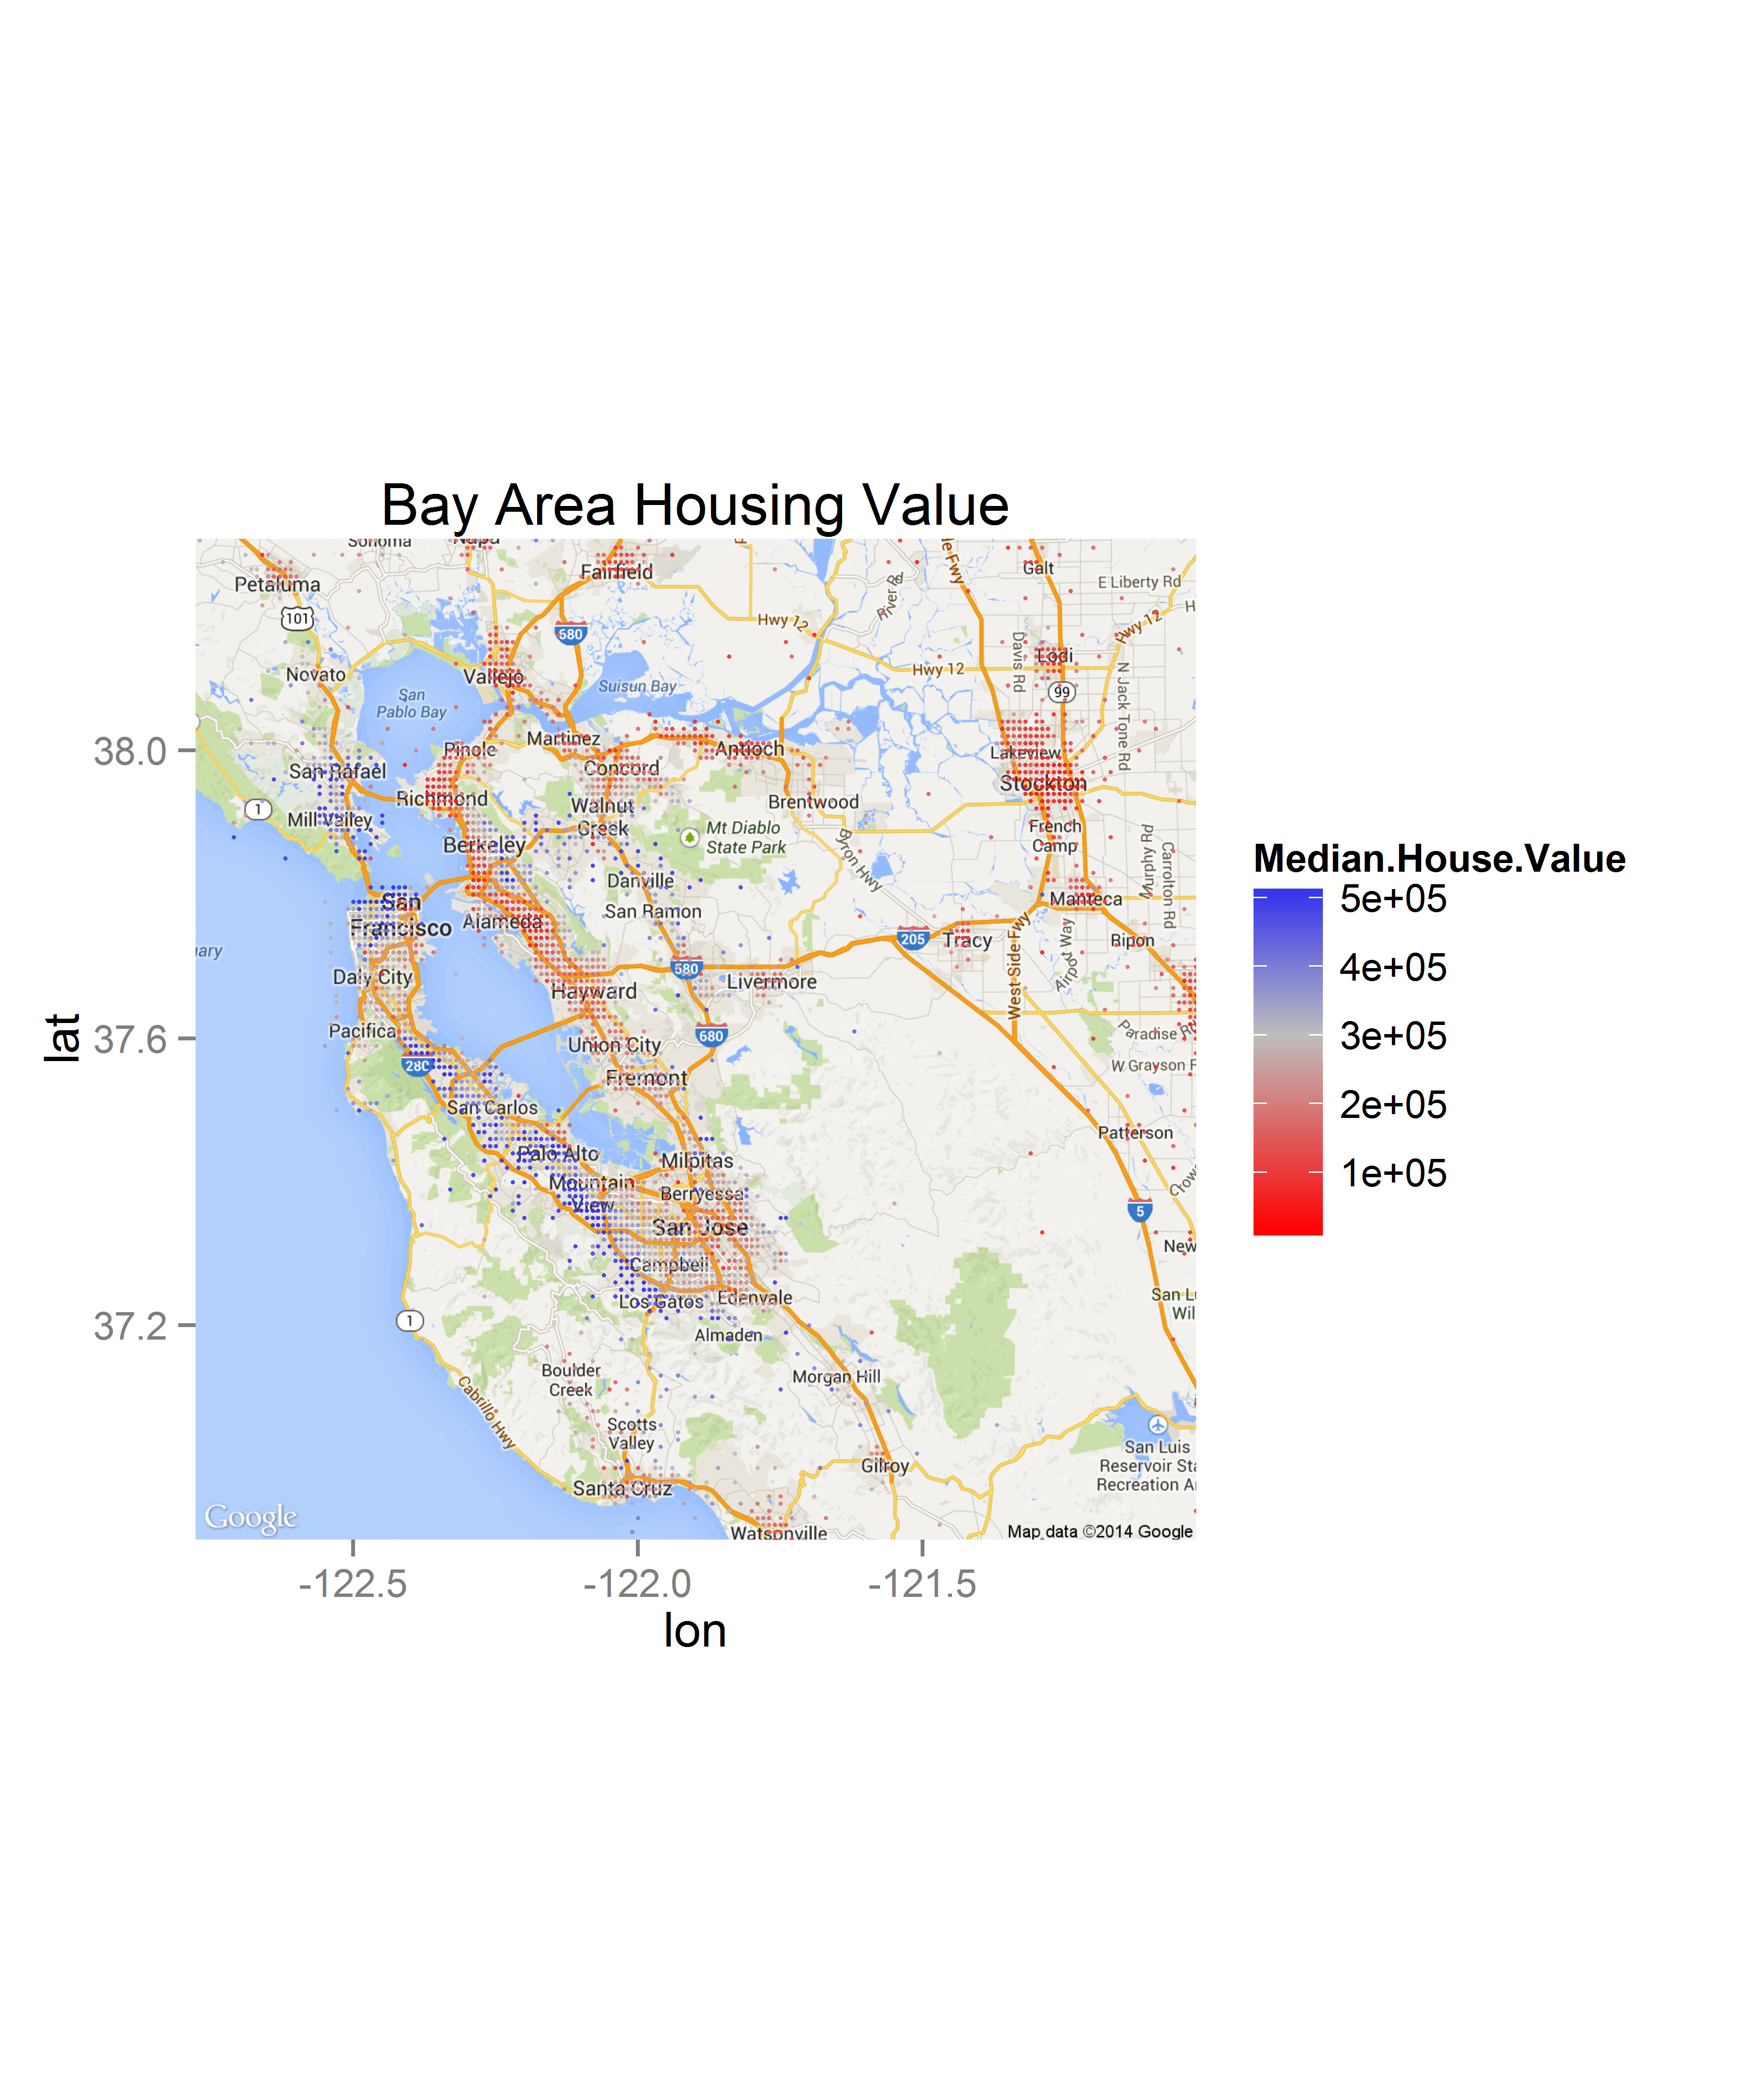
\includegraphics[scale=.54]{figures/bayarea.png}
\includegraphics[scale=.7]{figures/losangeles.png}
\end{figure}

The visualization helps us see how housing value is clustered in the state. As one might expect, rural areas generally have lower housing value than metropolitan areas. Within the metropolitan areas there are visible divisions as well. 

\newpage
Next we looked at space shuttle data taken from the UCI Machine Learning Repository. The goal was to predict the class given 8 predictors, with 43500 data points. Our logistic regression predicted whether or not the class was of type 1.  The description of the data set was very poor, however it matched our criterion for dimension, data points, and regression type. Because of the lack of sufficient description, few conclusions can be drawn from the data, but we can still test our Parsimony package.

Here is the summary of results using Parsimony:

\begin{tabular}{ | c | p{3cm} | p{3.3cm} | c  |}
\hline
Method&Parsimony (k=0.01) & Parsimony (k=0.05) & Significance Testing \\
\hline
Columns Deleted& V1,V3,V4,V6,V9 & V1,V2,V3,V4,V6,V9 & V4 \\
\hline
AIC & 8575.803 & 8728.906 & 8475.2 \\
\hline
\end{tabular}

We also tested the various methods against a validation training set. We looked at the probability of correctly identifying a class 1 or not class 1. Also if we identified something as class 1, what was the probability it was actually class 1 and the same for not class 1.

Here is a summary of the results:

\begin{tabular}{ | c | p{3cm} | p{3.3cm} | c  |}
\hline
Method&Parsimony (k=0.01) & Parsimony (k=0.05) & Significance Testing \\
\hline
P(Correct ID $|$ class 1) & 0.9862345 & 0.9861474 & 0.9864959 \\
\hline
P(Correct ID $|$ not class 1) & 0.9285242 & 0.9285242 & 0.9169424 \\
\hline
P(Correct ID $|$ guess class 1) & 0.981276 & 0.9812744 & 0.9783135 \\
\hline
P(Correct ID $|$ guess not class 1) & 0.9466937 & 0.9463744 & 0.9470267  \\
\hline
\end{tabular}

The results for the different methods are very close and it is hard to detect much difference in the accuracy levels. There were slightly fewer false positives and there was a slightly better detection of negatives for the Parsimony models. By simplifying the model, there is a possibility of increased accuracy during validation runs.
\\
\\


\subsection*{Census, 1994~\cite{census} (continuous and logistic, large $p$, large $n$)}
Census data which contains 32561 observations, 13 variable vectors and is based on 1994 Census. There are several categorical variables in this dataset. In order to accommodate regression modeling each categorical vector was split into 0-1 values vectors for each category. According to the website from which the dataset was taken was to predict whether a given person would be making over 50K a year.  Our parsimony function at k=0.1 eliminated all but one explanatory variable, which turned out to be "capital gain". 

\begin{verbatim}
Coefficients:
              Estimate Std. Error t value Pr(>|t|)    
(Intercept)  2.269e-01  2.334e-03   97.19   <2e-16 ***
capital.gain 1.293e-05  3.128e-07   41.34   <2e-16 ***
---

\end{verbatim}

This makes sense. If we were to look at only one column in order to predict in a person is making over 50K a year, the capital gain variable would be most informative. At k=0.01 there are many more explanatory variables that enhance the predictions:  "age", "education.num", "Exec.managerial", "Not.in.family", "Own.child", "Unmarried", "Wife", "capital.gain", "capital.loss", "hours.per.week".

\begin{verbatim}
Coefficients:
                  Estimate Std. Error t value Pr(>|t|)    
(Intercept)     -3.507e-01  1.284e-02 -27.323   <2e-16 ***
age              3.349e-03  1.602e-04  20.910   <2e-16 ***
education.num    4.195e-02  7.820e-04  53.650   <2e-16 ***
Exec.managerial  1.259e-01  6.036e-03  20.861   <2e-16 ***
Not.in.family   -2.774e-01  4.918e-03 -56.396   <2e-16 ***
Own.child       -2.439e-01  6.692e-03 -36.448   <2e-16 ***
Unmarried       -2.826e-01  6.702e-03 -42.167   <2e-16 ***
Wife             8.008e-02  9.369e-03   8.547   <2e-16 ***
capital.gain     8.576e-06  2.655e-07  32.304   <2e-16 ***
capital.loss     1.004e-04  4.836e-06  20.768   <2e-16 ***
hours.per.week   3.472e-03  1.665e-04  20.858   <2e-16 ***
---
\end{verbatim}

Another interesting variable that can be of interest for predictions is "sex", which can be only "Male" or "Female" in the scope of this census. With k=0.01 the following explanatory variables aren't eliminated: "Widowed", "Craft.repair", "Farming.fishing", "Handlers.cleaners", "Transport.moving", "Not.in.family", "Other.relative", "Own.child", "Unmarried", "Wife". Some of them make perfect sense, such as "Wife" variable. If somebody identified as a wife in 1994 Census it is very likely that the person was female. "Craft.repair", "Farming.fishing", and  "Transport.moving" variables makes sense too, and we expect to see a strong negative correlation between those jobs and being female in 1994.

\begin{verbatim}
Coefficients:
                   Estimate Std. Error t value Pr(>|t|)    
(Intercept)        0.072494   0.003360   21.57   <2e-16 ***
Widowed            0.253205   0.011353   22.30   <2e-16 ***
Craft.repair      -0.203757   0.005885  -34.62   <2e-16 ***
Farming.fishing   -0.224545   0.011122  -20.19   <2e-16 ***
Handlers.cleaners -0.268416   0.009565  -28.06   <2e-16 ***
Transport.moving  -0.208758   0.008911  -23.43   <2e-16 ***
Not.in.family      0.420779   0.004905   85.79   <2e-16 ***
Other.relative     0.412595   0.011385   36.24   <2e-16 ***
Own.child          0.420585   0.005736   73.33   <2e-16 ***
Unmarried          0.702012   0.006733  104.27   <2e-16 ***
Wife               0.936630   0.009252  101.23   <2e-16 ***
---

\end{verbatim}

Fitting the linear regression model to the data works as predicted, which supports out intuitive expectations of explanatory variable behavior. Naturally, the remaining variables are significant, however with large number of observations most variables are expected to be significant. 

With the continuously defined variable an interesting one to predict was "Age". After running our parsimony function with k=0.01, the variables that explain the variance in "Age" are "Self.emp.not.inc", "Assoc.acdm", "Never.married", "Widowed", "Own.child", "hours.per.week", "salary".   

\begin{verbatim}
Coefficients:
                   Estimate Std. Error t value Pr(>|t|)    
(Intercept)       44.927608   0.230145 195.215  < 2e-16 ***
Self.emp.not.inc   4.313808   0.224466  19.218  < 2e-16 ***
Assoc.acdm        -1.475503   0.335395  -4.399 1.09e-05 ***
Never.married    -10.851233   0.154146 -70.396  < 2e-16 ***
Widowed           16.070178   0.354766  45.298  < 2e-16 ***
Own.child         -8.221388   0.194804 -42.203  < 2e-16 ***
hours.per.week    -0.073794   0.005135 -14.371  < 2e-16 ***
salary             2.904975   0.150546  19.296  < 2e-16 ***
---
\end{verbatim}

 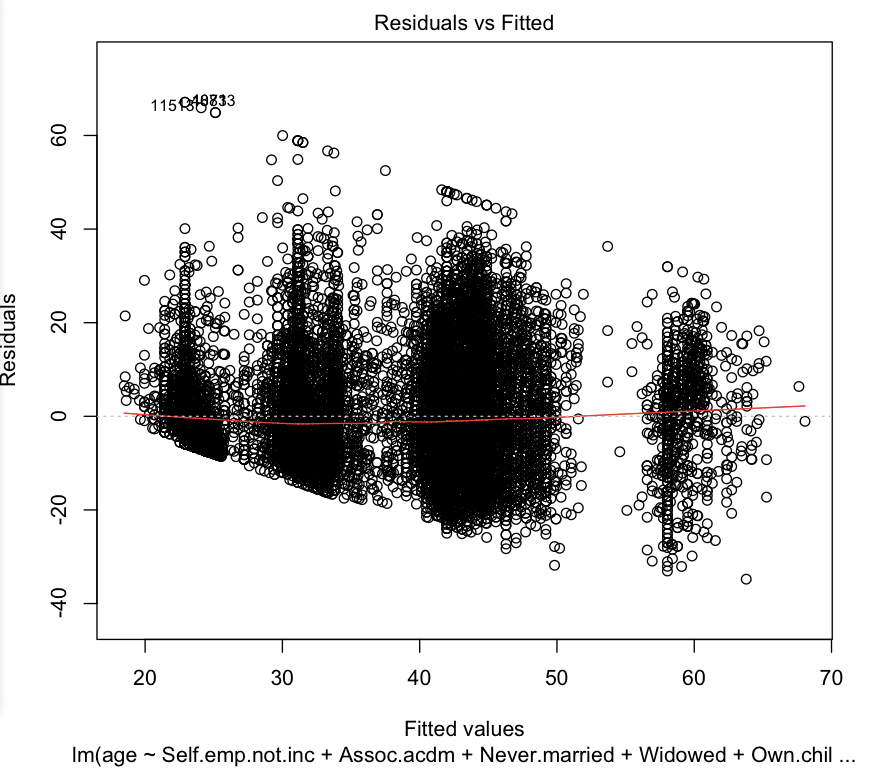
\includegraphics[scale=0.5]{figures/ageResidCensus.png}
 
 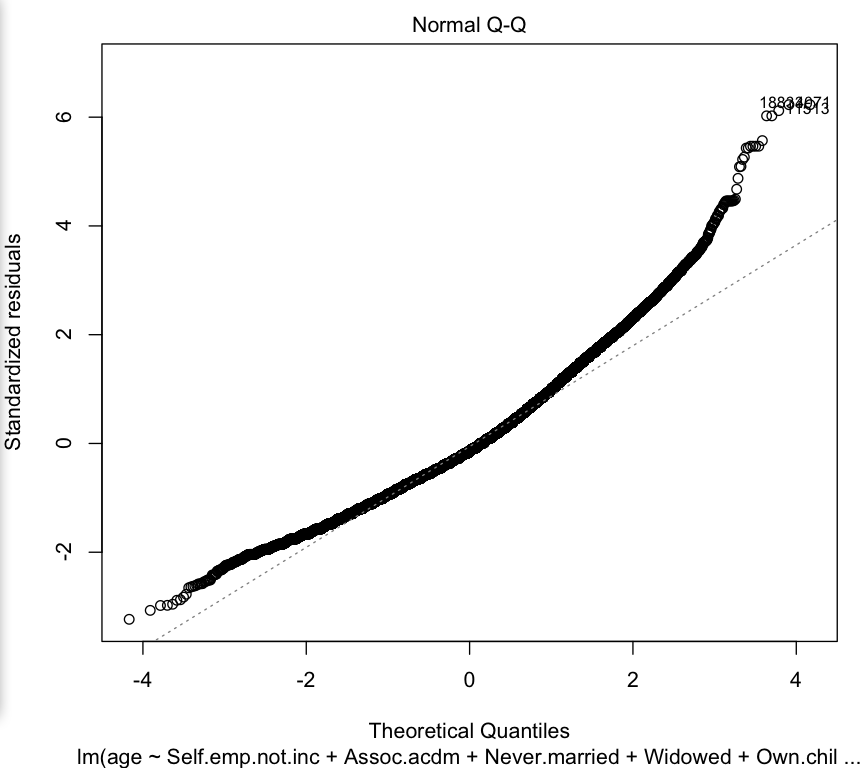
\includegraphics[scale=0.5]{figures/ageNormResidCensus.png}

 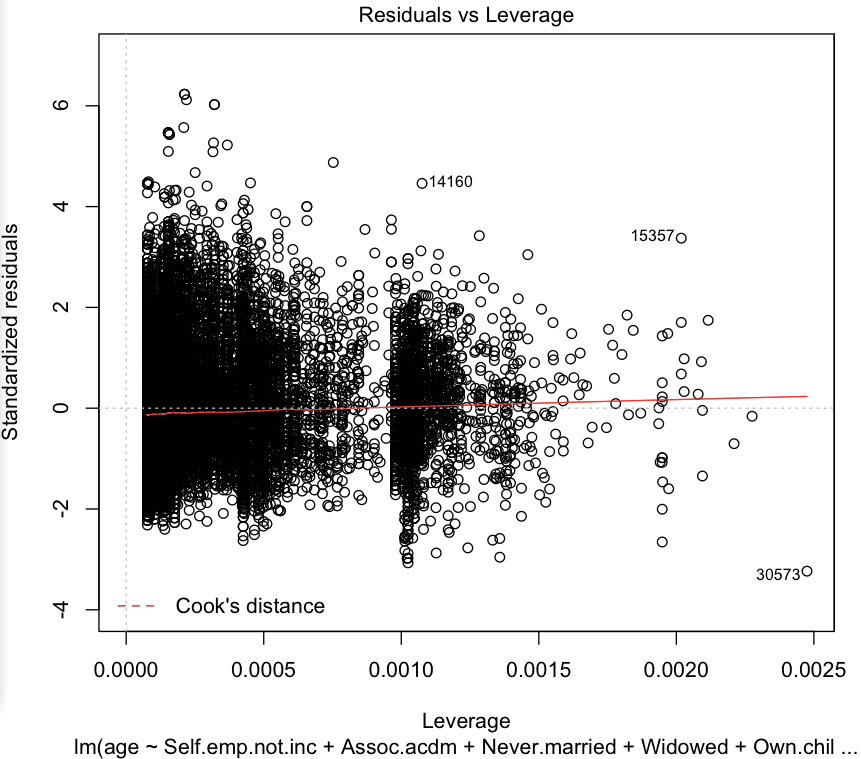
\includegraphics[scale=0.5]{figures/cookResidCensus.png}

In all of the performed analyses the countries of origin don't seem to play much role, or are too sparse to be good predictors of the outcome. Also it is interesting to point out that the education wasn't highly correlated with the variables of interest. It would be very interesting to compare these results with a more modern census information.

\newpage
% Begin John Chen's Section

% Parsimony: Price Prediction (Linear)

% Table of Parsimonious Variables
For the small n (n \textless 1000), large p (p \textgreater 15) case, we will use the automobile data set found on the UCI Machine Learning Repository.  The data set contains 193 instances, with 25 attributes each.  The attributes keep track of various specifications of cars that were attending a 1985 auto fair.  We will seek to determine which variables are the strongest predictors of a vehicle's price and safeness.

Here were the results of running prsm(): \\

\begin{center}
    \begin{tabular}{ | l |  p{4cm} |  p{4cm} | p{4cm} |}
    \hline
    Method & Parsimony (k = 0.01) & Parsimony (k = 0.05) & Significance Testing \\ \hline
    
    Columns Retained & ohcv, twelve-cylinders, engine.size, stroke, compression.ratio, peak.rpm & engine.size & bmw, dodge, `mercedes-benz`, mitsubishi, plymouth, porsche, saab, std, front, wheel.base, length, width, height, curb.weight, dohc, ohc, engine.size, peak.rpm\\ \hline
    
    AIC & 0.8676842 & 0.7888274 & 0.9308\\ \hline
    
    \end{tabular}
\end{center}

% Significance Testing Results
Summary of Significance Testing:\\
\begin{verbatim}
Coefficients:
              Estimate Std. Error t value Pr(>|t|)    
(Intercept) -5.360e+04  1.308e+04  -4.097 6.40e-05 ***
audi         1.628e+03  1.134e+03   1.436  0.15273    
bmw          8.537e+03  9.493e+02   8.992 4.02e-16 ***
dodge       -1.409e+03  9.491e+02  -1.484  0.13952    
mitsubishi  -2.507e+03  8.165e+02  -3.071  0.00248 ** 
plymouth    -1.390e+03  9.871e+02  -1.408  0.16096    
porsche      3.259e+03  2.497e+03   1.305  0.19345    
saab         2.994e+03  1.154e+03   2.593  0.01031 *  
std         -1.303e+03  5.721e+02  -2.277  0.02399 *  
front       -1.292e+04  2.976e+03  -4.343 2.38e-05 ***
wheel.base   1.644e+02  8.338e+01   1.972  0.05022 .  
length      -1.543e+02  4.576e+01  -3.372  0.00092 ***
width        9.632e+02  2.354e+02   4.092 6.55e-05 ***
height      -1.879e+01  1.279e+02  -0.147  0.88334    
curb.weight  3.625e+00  1.246e+00   2.909  0.00411 ** 
dohc         1.512e+03  8.983e+02   1.683  0.09422 .  
ohc          1.082e+03  5.095e+02   2.124  0.03511 *  
engine.size  9.950e+01  1.111e+01   8.954 5.10e-16 ***
peak.rpm     1.107e+00  4.399e-01   2.517  0.01274 *  
\end{verbatim}

\newpage

% Parsimony: Is this car relatively safe? (Logistic)

For the logistic regression case, we seek to find most effective variable, when it comes to determining how safe a car is.  In the original data set, each car is assigned a safety rating ranging from -3 to 3.  This range of values was converted into a discreet indicator variable - 1 if the car is relatively safe, having scored 1 or higher on the original scale.

% Table of Parsimonious Variables

Here are the results of running prsm():\\
\begin{center}
    \begin{tabular}{ | l |  p{4cm} |  p{4cm} | p{4cm} |}
    \hline
    Method & Parsimony (k = 0.01) & Parsimony (k = 0.05) & Significance Testing \\ \hline
    	
    Columns Retained & saab, toyota, volkswagen, turbo, two-doors, hatchback, sedan, 4wd, rwd, rear, wheel.base, length, width, height, curb.weight, l, ohc, ohcf ,ohcv, five-cylinders, four-cylinders, three-cylinders, twelve-cylinders, engine.size, 2bbl, idi, mfi, mpfi, spdi, bore, stroke, compression.ratio, horsepower, peak.rpm, city.mpg, highway.mpg & saab, toyota, volkswagen, turbo, two-doors, hatchback, sedan, 4wd, rwd, rear, wheel.base, length, width, height, curb.weight, l, ohc, ohcf ,ohcv, five-cylinders, four-cylinders, three-cylinders, twelve-cylinders, engine.size, 2bbl, idi, mfi, mpfi, spdi, bore, stroke, compression.ratio, horsepower, peak.rpm, city.mpg, highway.mpg & audi, saab, volkswagen, diesel, std, four-doors, 4wd, fwd, 1bbl\\ \hline
    
    AIC & 74 & 74 & 56\\ \hline
    
    \end{tabular}
\end{center}


% Significance Testing

\begin{verbatim}
Coefficients:
              Estimate Std. Error t value Pr(>|t|)    
(Intercept)   0.806479   0.074888  10.769  < 2e-16 ***
audi          0.590168   0.140289   4.207 4.05e-05 ***
saab          0.323690   0.140778   2.299 0.022618 *  
volkswagen    0.241768   0.105225   2.298 0.022715 *  
diesel       -0.165675   0.093946  -1.764 0.079483 .  
std          -0.002151   0.069947  -0.031 0.975495    
`four-doors` -0.674964   0.049956 -13.511  < 2e-16 ***
`4wd`        -0.038044   0.126373  -0.301 0.763724    
fwd           0.208747   0.054731   3.814 0.000187 ***
`1bbl`       -0.313088   0.106989  -2.926 0.003864 ** 

\end{verbatim}
 %End John Chen's Section
 

\section{Datasets Used}

\begin{thebibliography}{99}
    \bibitem{census} Dataset based on Census of 1994. $p=14 \rightarrow 110, n=32561$ \url{(https://archive.ics.uci.edu/ml/datasets/Adult} 
\end{thebibliography} 
 
\end{document}
